\section{PTS: Pure Type System}

\begin{definition}[PTS]
Un PTS $\cP $ esta definido por $\{ \cS, \cV, \cA, \cR\}$ donde

\begin{itemize}
    \item{$\cS$} es un conjunto sorts
    \item{$\cV$} es un conjunto de variables
    \item{$\cA$} es un conjunto no vacio de $\cS\times\cS$ llamados axiomas 
    \item{$\cR$} es un conjunto de $\cS\times\cS\times\cS$ llamadas $\Pi-Reglas$ 
\end{itemize}
\end{definition}

\begin{definition}[Pseudotérminos]
El conjunto T de pseudoterminos de un PTS $ \cP = \{ \cS, \cV, \cA, \cR\}$ 
es el menor conjunto que satisface lo siguiente:
\begin{itemize}
    \item{} $\cS \cup \cV \subset \cT$
    \item{} Si $a \in \cT$ y $b \in \cT$ entonces $ab \in\cT$
    \item{} Si $A \in \cT$,  $B \in \cT$  y $x \in \cV$  entonces $(\lambda x:A.B) \in\cT$
    \item{} Si $A \in \cT$,  $B \in \cT$  y $x \in \cV$  entonces $(\Pi x:A.B) \in\cT$
\end{itemize}
\end{definition}

\begin{definition}[PTS funcional]
Un PTS se dice \emph{funcional} si
\begin{itemize}
\item $\langle s_1, s \rangle \in \cA$ y $\langle s_1, s'\rangle \in \cA$ implica $s = s'$;
\item $\langle s_1, s_2, s\rangle \in \cR$ y $\langle s_1, s_2, s' \rangle \in \cR$ implica $s = s'$.
\end{itemize}
\end{definition}
\begin{definition}[PTS full]
Un PTS se dice \emph{full} si para todo $s_1, s_2 \in \cS$
existe un $s_3 \in \cS$ con $\langle s_1, s_2, s_3 \rangle \in \cR$.
\end{definition}

\begin{definition}[PTS semifull]
Un PTS se dice \emph{semi-full} si para todo $s_1 \in \cS$
$\exists s_2, s_3 [\langle s_1, s_2, s_3 \rangle \in \cR ] \Rightarrow \forall s_2 \exists s_3 [\langle s_1, s_2, s_3 \rangle \in \cR ]$
\end{definition}


\begin{lemma}
 PTS full $\Rightarrow$ PTS semi full ??


 PTS funcional $\Rightarrow$ PTS full o semi full??
\end{lemma}

\begin{definition}[Relación $\vdash$]
Definimos a la relacion $\vdash$, con $\vdash \subseteq \mathcal{C}\times\cT\times\cT$ como
la menor relación que cumple:


\[
\begin{array}{llcr}
	(Srt) & &\infer{\emptyset \vdash s_{1} : s_{2}}{} & (s_{1},s_{2}) \in\cA \\ \\
	(Var) & &\infer{\Gamma, x:A \vdash x:A}{\Gamma\vdash A:s} & \\ \\
	(Wk)  & &\infer{\Gamma, x:A \vdash b:B}{\Gamma\vdash b:B & \Gamma\vdash A:s} & b\in\cS\cup\cV \\ \\
	(Pi)  & &\infer{\Gamma \vdash \Pi x:A.B : s_{3}}{\Gamma\vdash A:s_{1} & \Gamma, x:A \vdash B:s_{2}} &  (s_1,s_2,s_3)\in\cR\\ \\
	(Lda) & &\infer{\Gamma \vdash \lambda a:A.b : \Pi x:A.B }{\Gamma\vdash A:s_{1} & \Gamma, x:A \vdash b:B &\Gamma, x:A \vdash B:s_{2}} &  (s_1,s_2,s_3)\in\cR\\ \\
	(App) & &\infer{\Gamma \vdash a b : A[x:= b] }{\Gamma\vdash a : \Pi x:B.A & \Gamma \vdash b:B} &  \\ \\
	(Cnv) & &\infer{\Gamma \vdash a:B}{\Gamma\vdash a:A & \Gamma\vdash B:s} & A \simeq B \\ \\
	
\end{array}
\]

\end{definition}

\subsection{Ejemplos}

Sea $\cS = \{\Prop, \Type\}$ y $\cA = \{(\Prop : \Type)\}$ tenemos que

\begin{itemize}
    \item $\lambda^{\rightarrow}$ es el PTS con $(\cS, \cV, \cA, \cR_{1})$
    \item $\lambda \Pi$ es el PTS con $(\cS, \cV, \cA, \cR_{2})$
    \item $\lambda C$ es el PTS con $(\cS, \cV, \cA, \cR_{3})$
\end{itemize}

\subsection{Optimización}

Podemos introducir un modificación a $\vdash$ orientada a la implementación. En lugar de tener que usar $Wk$ para
obtener un contexto valido podemos asumir que el mismo es valido. De esta forma las reglas $\vdash_{vtyp}$ se definiría de la 
siguiente manera:

\begin{definition}[Relación $\vdash_{vtyp}$]
Definimos a la relacion $\vdash_{vtyp}$, con $\vdash_{vtyp} \subseteq \mathcal{C}\times\cT\times\cT$ como
la menor relación que cumple:


\[
\begin{array}{llcr}
	(Srt-vtyp) & &\infer{\Gamma \vdash_{vtyp} s_{1} : s_{2}}{} & (s_{1},s_{2}) \in\cA \\ \\ 
	(Var-vtyp) & &\infer{\Gamma \vdash_{vtyp} x : A}{} & x:A \in\Gamma \\ \\
	(Pi-vtyp)  & &\infer{\Gamma \vdash_{vtyp} \Pi x:A.B : s_{3}}{\Gamma\vdash_{vtyp} A:s_{1} & \Gamma, x:A \vdash_{vtyp} B:s_{2}} &  (s_1,s_2,s_3)\in\cR\\ \\
               & &                                             & x \not\in dom(\Gamma)\\
	(Lda-vtyp) & &\infer{\Gamma \vdash_{vtyp} \lambda a:A.b : \Pi x:A.B }{\Gamma\vdash_{vtyp} A:s_{1} & \Gamma, x:A \vdash_{vtyp} b:B &\Gamma, x:A \vdash B:s_{2}} &  (s_1,s_2,s_3)\in\cR\\ \\
               & &                                             & x \not\in dom(\Gamma)\\
	(App-vtyp) & &\infer{\Gamma \vdash_{vtyp} a b : A[x:= b] }{\Gamma\vdash_{vtyp} a : \Pi x:B.A & \Gamma \vdash_{vtyp} b:B} &  \\ \\
	(Cnv-vtyp) & &\infer{\Gamma \vdash_{vtyp} a:B}{\Gamma\vdash_{vtyp} a:A & \Gamma\vdash_{vtyp} B:s} & A \simeq B \\ \\
	
\end{array}
\]

\end{definition}

PASAR A LATEX

\begin{figure}[h]
\centering
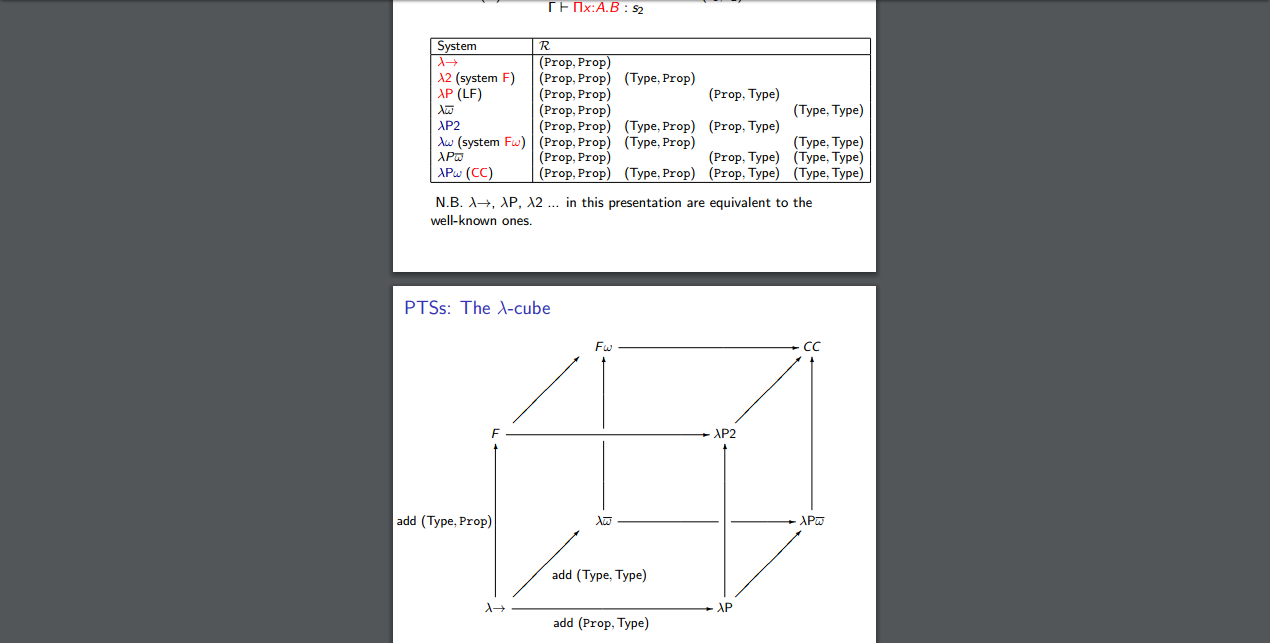
\includegraphics[width=\textwidth]{pts_examples}
\end{figure}

\begin{figure}[h]
\centering
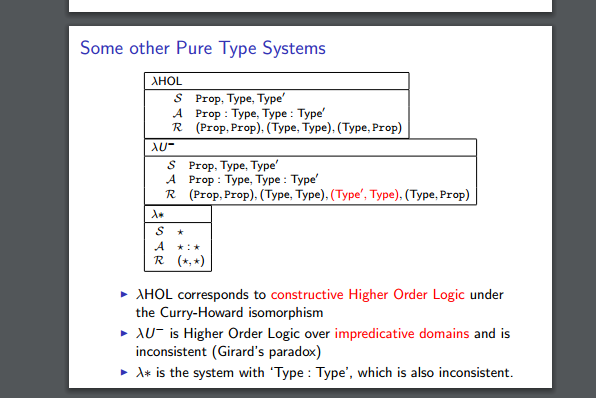
\includegraphics[width=\textwidth]{pts_examples2}
\end{figure}

\begin{definition}[Relación $\vdash_{vctx}$]
Definimos a la relacion $\vdash_{vctx}$, con el menor predicado sobre $\mathcal{C}$ que satisface:

\[
\begin{array}{llcr}
	(Nil-vctx)  & &\infer{\emptyset \vdash_{vctx}}{} \\ \\ 
	(Cons-vctx) & &\infer{\Gamma, x:A \vdash_{vctx}}{\Gamma \vdash_{vctx} & \Gamma \vdash_{vtyp} A : s} \\ \\ 
	

	
\end{array}
\]

\begin{lemma}{Equivalencia de $\vdash$ y $\vdash_{vtyp}$}

\begin{equation}
\Gamma \vdash a : A \Leftrightarrow \Gamma \vdash_{vctx} \land \Gamma \vdash_{vtyp} a:A
\end{equation}
\end{lemma}

\end{definition}


\section{PTS Semifull}

\begin{definition}[$\vdash_sf$]

$\vdash_sf \subseteq \mathcal{C}\times\cT\times\cT$ es la menor relación que satisface las relgas de $\vdash$ pero
se reemplaza la regla $lda$ por

\[
\begin{array}{llcr}
	(Lda1-sf) & &\infer{\Gamma \vdash_{sf} \lambda x:A.b : \Pi x:A.B}{\Gamma \vdash_{sf} A:s_1& \Gamma x:A \vdash_{sf} b : B} & \langle s_1,s_2,s_3 \rangle \in \cR  \\  
	          & &                                                                                                             & B \in \cS  \\ 
	(Lda2-sf) & &\infer{\Gamma \vdash_{sf} \lambda x:A.b : \Pi x:A.s_b}{\Gamma \vdash_{sf} A:s_1& \Gamma x:A \vdash_{sf} b : s_b} & \langle s_1,s_2,s_3 \rangle \in \cR \\ 
	          & &                                                                                                             & \langle s_b, s_4 \rangle \in \cA  \\ 
	

	
\end{array}
\]


\end{definition}

\begin{lemma}{Equivalencia entre $\vdash$ y $\vdash_{sf}$}
Dado un PTS semifull tenemos que

\begin{equation}
\Gamma \vdash a : A \Leftrightarrow \Gamma \vdash_{sf} a: A
\end{equation}

\end{lemma}



\begin{definition}[$\vdash_sfnsd$]
Usando $\vdash_{sf}$ podemos de definir una nueva relación casi dirigida por sintaxis, $\vdash_{sfnsd} \subseteq \mathcal{C}\times\cT\times\cT$ es la
menor relacion que satisface:


\[
\begin{array}{llcr}
	(Srt-sfnsd) & &\infer{\emptyset \vdash_{sfnsd} s_{1} : s_{2}}{} & (s_{1},s_{2}) \in\cA \\ \\
	(Var-sfnsd) & &\infer{\Gamma, x:A \vdash_{sfnsd} x:A}{\Gamma\vdash_{sfnsd} A:\twoheadrightarrow s} & \\ \\
	(Wk-sfnsd)  & &\infer{\Gamma, x:A \vdash_{sfnsd} b:B}{\Gamma\vdash_{sfnsd} b:B & \Gamma\vdash_{sfnsd} A:\twoheadrightarrow s} & b\in\cS\cup\cV \\ \\
	(Pi-sfnsd)  & &\infer{\Gamma \vdash_{sfnsd} \Pi x:A.B : s_{3}}{\Gamma\vdash_{sfnsd} A:\twoheadrightarrow s_{1} & \Gamma, x:A \vdash_{sfnsd} B:\twoheadrightarrow s_{2}} &  (s_1,s_2,s_3)\in\cR\\ \\

	(Lda1-sfnsd) & &\infer{\Gamma \vdash_{sfnsd} \lambda x:A.b : \Pi x:A.B}{\Gamma \vdash_{sfnsd} A:\twoheadrightarrow s_1& \Gamma x:A \vdash_{sfnsd} b : B} & \langle s_1,s_2,s_3 \rangle \in \cR  \\  
	          & &                                                                                                             & B \in \cS  \\ 
	(Lda2-sfnsd) & &\infer{\Gamma \vdash_{sfnsd} \lambda x:A.b : \Pi x:A.s_b}{\Gamma \vdash_{sfnsd} A:\twoheadrightarrow s_1& \Gamma x:A \vdash_{sfnsd} b : s_b} & \langle s_1,s_2,s_3 \rangle \in \cR \\ 
	          & &                                                                                                             & \langle s_b, s_4 \rangle \in \cA  \\ 

	(App-sfnsd) & &\infer{\Gamma \vdash_{sfnsd} a b : A[x:= b] }{\Gamma\vdash_{sfnsd} a : \twoheadrightarrow^{wh} \Pi x:B_0 .A & \Gamma \vdash_{sfnsd} b:B_1} & B_0 \simeq B_1  \\ \\
	
\end{array}
\]



\end{definition}

\begin{lemma}{Equivalencia entre $\vdash_{sf}$ y $\vdash_{sfnsd}$}
Dado un PTS semifull tenemos que 

\begin{itemize}
    \item Si $\Gamma \vdash_{sfnsd} a : A$ entonces $\Gamma \vdash_{sf} a:A$
    \item Si $\Gamma \vdash_{sf} a : A$ entonces $\exists A_0 | \Gamma \vdash_{sfnsd} a : A_0 \land A_0 \simeq A$
    
\end{itemize}

\end{lemma}

\begin{lemma}
Si tenemos un PTS semifull y funcional entonces $\vdash_{sfnsd}$ son reglas dirigidas por sintaxis
\end{lemma}
